\documentclass[border=0.2cm]{standalone}
\usepackage{tikz}
\usetikzlibrary{automata, arrows.meta, positioning}

\begin{document}

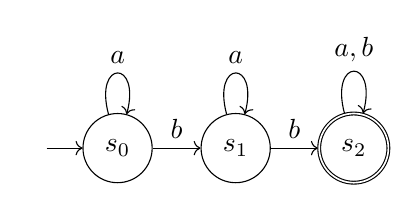
\begin{tikzpicture} [
    every initial by arrow/.style = {-To},
    every loop/.style = {-To}]
    % \draw [help lines] (-1,-1) grid (5,1);
    \node (q0) [state, 
        initial, 
        initial text={}] at (0,0) {$s_{0}$};
    \node (q1) [state] at (1.5,0) {$s_{1}$};
    \node (q2) [state, 
        accepting] at (3.0,0) {$s_{2}$};
    
    \path [-To]
        (q0) edge node [above] {$b$} (q1)
        (q1) edge node [above] {$b$} (q2)
        (q0) edge [loop above] node {$a$} ()
        (q1) edge [loop above] node {$a$} ()
        (q2) edge [loop above] node {$a,b$} ();
\end{tikzpicture}

\end{document}